\documentclass{article}

\usepackage{indentfirst}
\usepackage{graphicx}
\usepackage{listings}
\usepackage{fancyhdr}
\usepackage{hyperref}
\usepackage{amsmath}
\usepackage{amssymb}

\title{CIC202 - Programação Concorrente: Trabalho 1 \\
        \large \textbf{Sincronização de Processos:} A Caverna dos Sableyes}
\author{Guilherme da Rocha Cunha - 221030007}
\date{2024.1}

\begin{document}

\pagestyle{fancy}

\maketitle

\begin{figure}[ht]
        \centering
        
\includegraphics[width=.5\textwidth]{imagens/as_vert_cor.jpg}
\end{figure}

\newpage

\fancyhead{}
\fancyhead[L]{\textbf{Sincronização de Processos:} A Caverna dos Sableyes}
\fancyfoot[C]{\thepage}


\renewcommand*\contentsname{Sumário}
\tableofcontents

\newpage

\section{Introdução}
O trabalho consiste na aplicação dos conhecimentos adquiridos na disciplina "CIC202 - Programação Concorrente". Nele é apresentado o problema de comunicação de processos atráves de uma memória compartilhada, "A Caverna dos Sableyes", e sua solução utilizando a biblioteca POSIX Pthereads na linguagem C.

\section{Formalização do Problema: A Caverna dos Sableyes}
Sableyes são uma espécie de pokemon de pele roxa, garras e dentes afiados, que se alimentam de pedras preciosas e moram no interior de cavernas.

\begin{figure}[ht]
        \centering
        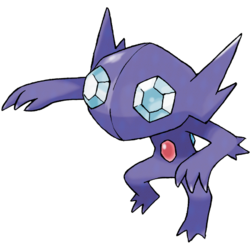
\includegraphics[width = .25\textwidth]{imagens/sableye.png}
        \caption{Sableye}
\end{figure}

É comum deles perambularem pelas câmaras das cavernas em que habitam em busca de joias e carbinks (suas presas), principalmente depois de um terremoto. Após um terremoto, as câmaras das cavernas têm uma chance de revelar joias que até então estavam enterradas ou presas no teto da caverna.

O problema consiste na simulação da busca dos sableyes por alimento. Há $n$ sableyes e $m$ câmaras na caverna, onde cada câmara possui um quantidade $j_i$ de joias preciosas reveladas $(1 \leq i \leq m)$.

Se um sableye está na $i$-ésima câmara, ele vai tentar comer até $j_i$ joias. No caso de não houver joias, ele vai embora e tenta procurar por comida em outro lugar.

Em um determinado momento, ocorrerá um terremoto na caverna. Para cada câmara $i$, o terremoto irá revelar $k_i$ novas joias. Enquanto estiver ocorrendo um terremoto, nenhum sableye estará procurando por comida.

\section{Descrição do Algoritmo}

\section{Conclusão}

\section{Referências}

\end{document}